\documentclass[10pt,journal,compsoc]{IEEEtran}

\usepackage{amsmath,amssymb,amsfonts}
\usepackage{algorithmic}
\usepackage{graphicx}
\usepackage{textcomp}
\usepackage{xcolor}
\usepackage{booktabs}
\usepackage{multirow}
\usepackage{url}
\usepackage{hyperref}
\usepackage{cite}

\hypersetup{
    colorlinks=true,
    linkcolor=blue,
    filecolor=magenta,      
    urlcolor=cyan,
    citecolor=blue,
}

\begin{document}

\title{A Hybrid AML Detection and Evidence-Grounded SAR Generation Framework with Tamper-Evident Audit Logging}

\author{Author~1,
        Author~2,
        and~Author~3% <-this % stops a space
\IEEEcompsocitemizethanks{\IEEEcompsocthanksitem The authors are with the Department of Computer Science and Engineering, Institution Placeholder.\protect\\
E-mail: corresponding-author@institution.edu
}}

\IEEEtitleabstractindextext{%
\begin{abstract}
Anti-Money Laundering (AML) monitoring in contemporary financial institutions is severely constrained by three systemic vulnerabilities: extreme false-positive alert rates in threshold rules, siloed analytical tools that fail to capture multi-hop fund routing, and the operational bottleneck of manually drafting Suspicious Activity Reports (SARs). This paper presents an integrated, end-to-end AML investigation-support framework that bridges suspicious activity detection, automated evidence enrichment, retrieval-augmented narrative generation, and tamper-evident audit logging. The detection architecture unifies three complementary paradigms: a deterministic statutory rules engine, an unsupervised 16-feature tabular Isolation Forest anomaly detector, and a directed multigraph structural detector identifying rapid pass-through, circular funds routing, and high-degree aggregation hubs. Flagged cases undergo automated transaction-history enrichment and are synthesized into structured, five-part regulatory SAR narratives via a local Retrieval-Augmented Generation (RAG) pipeline incorporating regulatory guidance (FATF, PMLA, FIU-IND) and privacy-preserving Personally Identifiable Information (PII) masking. To enforce accountability without decentralized blockchain overhead, every investigation milestone and review decision is cryptographically anchored in a sequential SHA-256 hash-chained ledger. Evaluated on a frozen, chronological synthetic benchmark ($N=1{,}474$ transactions, 39 accounts, 30 customers), the hybrid detector achieves a test recall of $0.9915$ and F1-score of $0.9249$, while Isolation Forest achieves a superior area under the precision-recall curve (PR-AUC of $0.9369$ vs. $0.9156$). At tight operational false-positive rate budgets ($\le 3\%$), the hybrid model delivers superior precision ($95.65\%$ vs. $88.89\%$) through cross-detector corroboration. The automated SAR rubric achieves an average score of $80.0/100$ with zero PII leakage, and the audit ledger detects $100\%$ of injected database tampering events. We discuss framework limitations, including synthetic-to-real domain shift and single-node ledger trust boundaries.
\end{abstract}

\begin{IEEEkeywords}
Anti-Money Laundering, Suspicious Activity Reporting, Isolation Forest, Graph Analytics, Hybrid Detection, Retrieval-Augmented Generation, Synthetic Financial Data, Explainable AI, Tamper-Evident Auditing.
\end{IEEEkeywords}}

\maketitle
\IEEEdisplaynontitleabstractindextext
\IEEEpeerreviewmaketitle

\section{Introduction}
\IEEEPARstart{F}{inancial} institutions globally operate under stringent statutory mandates to monitor transactions and file Suspicious Activity Reports (SARs) with domestic financial intelligence units, such as FinCEN in the United States and FIU-IND in India under the Prevention of Money-Laundering Act (PMLA) \cite{fatf2012guidance, fincen2020sar, pmla2002act}. Despite massive compliance expenditures, operational AML systems remain plagued by high false-alarm rates exceeding $90\%$, driven primarily by brittle, single-transaction threshold rules \cite{chen2023machine}. These legacy filters routinely fail to recognize sophisticated money laundering typologies---such as smurfing (structuring payments beneath statutory reporting thresholds), rapid pass-through routing across intermediary mule accounts, and closed circular flow networks designed to simulate legitimate trade \cite{jullum2020detecting}.

Machine learning approaches, particularly statistical anomaly detectors like Isolation Forest \cite{liu2008isolation}, offer adaptive detection of multi-dimensional feature deviations. However, tabular algorithms treat transactions as independent and identically distributed observations, remaining blind to complex graph-structural subgraphs formed across multiple entities and banking accounts \cite{weber2019anti}. Conversely, graph analysis algorithms identify topological motifs (such as directed cycles and fan-in/fan-out star topologies), but introduce computational bottlenecks and high false-alarm burdens when benign commercial hubs (e.g., e-commerce payment aggregators) coincide with structural patterns \cite{hagberg2008exploring}.

Crucially, detection represents only the initial phase of the AML compliance lifecycle. Once an alert triggers, human compliance analysts spend hours assembling fragmented transaction records, cross-referencing account histories, establishing entity relationships, and drafting narrative reports that satisfy strict legal and regulatory filing standards \cite{fincen2020sar}. Recent advancements in Large Language Models (LLMs) present compelling opportunities to accelerate narrative drafting. However, deploying generative models in regulatory compliance introduces severe risks of factual hallucination, unverified assertions, customer privacy violations, and lack of statutory grounding. Furthermore, regulatory scrutiny requires an unalterable audit trail establishing exactly which analytical findings, evidence records, and human review steps informed each SAR filing \cite{crosby2009efficient, haber1991time}.

To address these interconnected challenges, this paper presents an integrated, open-source AML investigation-support framework that bridges detection, investigation, narrative preparation, human review, and audit integrity. The framework does not purport to autonomously prove criminal guilt; rather, it provides a deterministic, defensible investigation workbench for human compliance officers.

\section{Related Work}
\subsection{Rule-Based Monitoring and Tabular Machine Learning}
Traditional transaction monitoring systems rely predominantly on deterministic rule engines encoding statutory thresholds, such as cash transactions exceeding INR 1,000,000 or USD 10,000, and transfers involving high-risk jurisdictions \cite{fatf2012guidance, rbi2016kyc}. While transparent, rule-based systems are vulnerable to adversarial adaptation, generating massive false-positive burdens that overwhelm investigative teams \cite{chen2023machine}.

To improve flexibility, supervised and unsupervised machine learning methods have been applied to tabular financial data \cite{chandola2009anomaly}. Isolation Forest, introduced by Liu et al. \cite{liu2008isolation, liu2012isolation}, isolates anomalous instances by randomly partitioning feature space using axis-aligned orthogonal cuts. Because anomalies require fewer splits to isolate than normal clustering points, tree path length serves as a robust proxy for abnormality. Although effective for high-dimensional point outliers, tabular algorithms do not explicitly model relational topology between transaction counterparties.

\subsection{Graph Analytics and Network Topologies}
Financial transactions naturally form directed, weighted, dynamic multigraphs where nodes represent account holders and edges represent payment flows \cite{weber2019anti}. Prior research has demonstrated that illicit funds movement frequently exhibits distinct topological motifs: rapid pass-through layering, circular round-tripping loops, and fan-in/fan-out structures \cite{jullum2020detecting}. While Graph Convolutional Networks (GCNs) have shown promise on cryptocurrency benchmarks \cite{weber2019anti}, exact subgraph motif mining using libraries like NetworkX \cite{hagberg2008exploring} provides deterministic, explainable evidence required by banking regulators.

\subsection{Retrieval-Augmented Generation and Regulatory Compliance}
Retrieval-Augmented Generation (RAG), formulated by Lewis et al. \cite{lewis2020retrieval}, couples parametric sequence-to-sequence models with non-parametric dense vector indices. In high-stakes regulatory applications, RAG anchors generated text in verified source documents, mitigating hallucinations \cite{reimers2019sentence}. FinCEN guidelines require SAR narratives to comprehensively address the ``who, what, when, where, why, and how'' while strictly avoiding prejudicial assertions of legal guilt \cite{fincen2020sar}.

\subsection{Cryptographic Audit Trails vs. Blockchain}
To ensure evidentiary integrity in legal proceedings, financial monitoring systems require tamper-evident logging \cite{crosby2009efficient}. While popular discourse frequently advocates for distributed blockchain ledgers, enterprise banking deployments face severe privacy, latency, and operational constraints with public blockchains. Classic cryptographic mechanisms---specifically sequential SHA-256 hash chains \cite{haber1991time} and forward-secure logging architectures \cite{bellare2003forward}---provide rigorous mathematical proof of append-only integrity without consensus complexity.

\section{Problem Formulation}
Let a financial transaction record $T_i$ be defined by the tuple:
\begin{equation}
T_i = \left(\text{id}_i, \text{src}_i, \text{dst}_i, a_i, t_i, m_i\right)
\end{equation}
where $\text{id}_i \in \mathcal{T}$ is a unique transaction identifier, $\text{src}_i \in \mathcal{A}$ is the source account, $\text{dst}_i \in \mathcal{A}$ is the destination counterparty account, $a_i \in \mathbb{R}^+$ denotes the transaction amount (denominated in INR), $t_i \in \mathcal{T}_{\text{time}}$ is the transaction execution timestamp (UTC), and $m_i$ represents categorical metadata including transaction channel (e.g., UPI, NEFT, RTGS, SWIFT), country code, and currency.

Enforcing temporal causality, for any target transaction $T_i$ evaluated as of time $t_i$, the historical baseline context is strictly restricted to:
\begin{equation}
\mathcal{H}(T_i) = \{ T_j \in \mathcal{T} \mid \text{src}_j = \text{src}_i \land t_j < t_i \}
\end{equation}
A deterministic feature extraction function $\Phi: (T_i, \mathcal{H}(T_i)) \to \mathbb{R}^{16}$ extracts tabular features capturing monetary scale, robust Median Absolute Deviation (MAD) spread, rolling velocity windows ($24\text{h}, 7\text{d}, 30\text{d}$), counterparty diversity, and cyclical temporal encodings.

Transactions occurring within a sliding temporal window $W$ are modeled as a directed multigraph $G_W = (V, E)$, where $V \subseteq \mathcal{A}$ and $e_k = (\text{src}_k, \text{dst}_k, k)$ with weight $a_k$ and timestamp $t_k$.

The hybrid risk aggregator computes a composite score $S_{\text{hybrid}}(T_i)$:
\begin{equation}
S_{\text{hybrid}}(T_i) = \frac{\sum_{m \in \mathcal{M}_{\text{act}}} w_m S_m(T_i)}{\sum_{m \in \mathcal{M}_{\text{act}}} w_m}
\end{equation}
where $\mathbf{w} = (0.35, 0.35, 0.30)$ for Rules, Isolation Forest, and Graph detectors respectively. An operational threshold $\tau \in [0.0, 1.0]$, calibrated strictly on validation data, maps continuous risk into a triage decision:
\begin{equation}
Y_{\text{pred}}(T_i) = \begin{cases} 1 \quad (\text{ALERT / SAR Eligible}), & \text{if } S_{\text{hybrid}}(T_i) \ge \tau \\ 0 \quad (\text{BENIGN / Pass}), & \text{if } S_{\text{hybrid}}(T_i) < \tau \end{cases}
\end{equation}

\section{Overall System Architecture}
The framework comprises four cohesive layers operating within a modular FastAPI and database backend (Fig.~\ref{fig:arch}):
\begin{enumerate}
    \item \textbf{Ingestion \& Preprocessing}: Ingests transactions, enforces chronological sorting, validates Pydantic contracts, and updates customer profile baselines with zero lookahead.
    \item \textbf{Multi-Detector Engine}: Concurrently runs rules, tabular Isolation Forest, and multigraph motif analysis, with dynamic weight renormalization in degraded mode.
    \item \textbf{Investigation \& RAG Narrative Generation}: Enriches flagged cases with historical context, retrieves PMLA/FATF guidance from ChromaDB using `all-MiniLM-L6-v2`, masks PII, and invokes a local LLM (Ollama `phi3:mini`) to generate a five-part SAR.
    \item \textbf{Human Review \& Tamper-Evident Ledger}: Manages analyst RBAC triage, generates certified ReportLab PDF filings, and cryptographically commits all state changes to a sequential SHA-256 hash chain.
\end{enumerate}

\begin{figure*}[t]
\centering
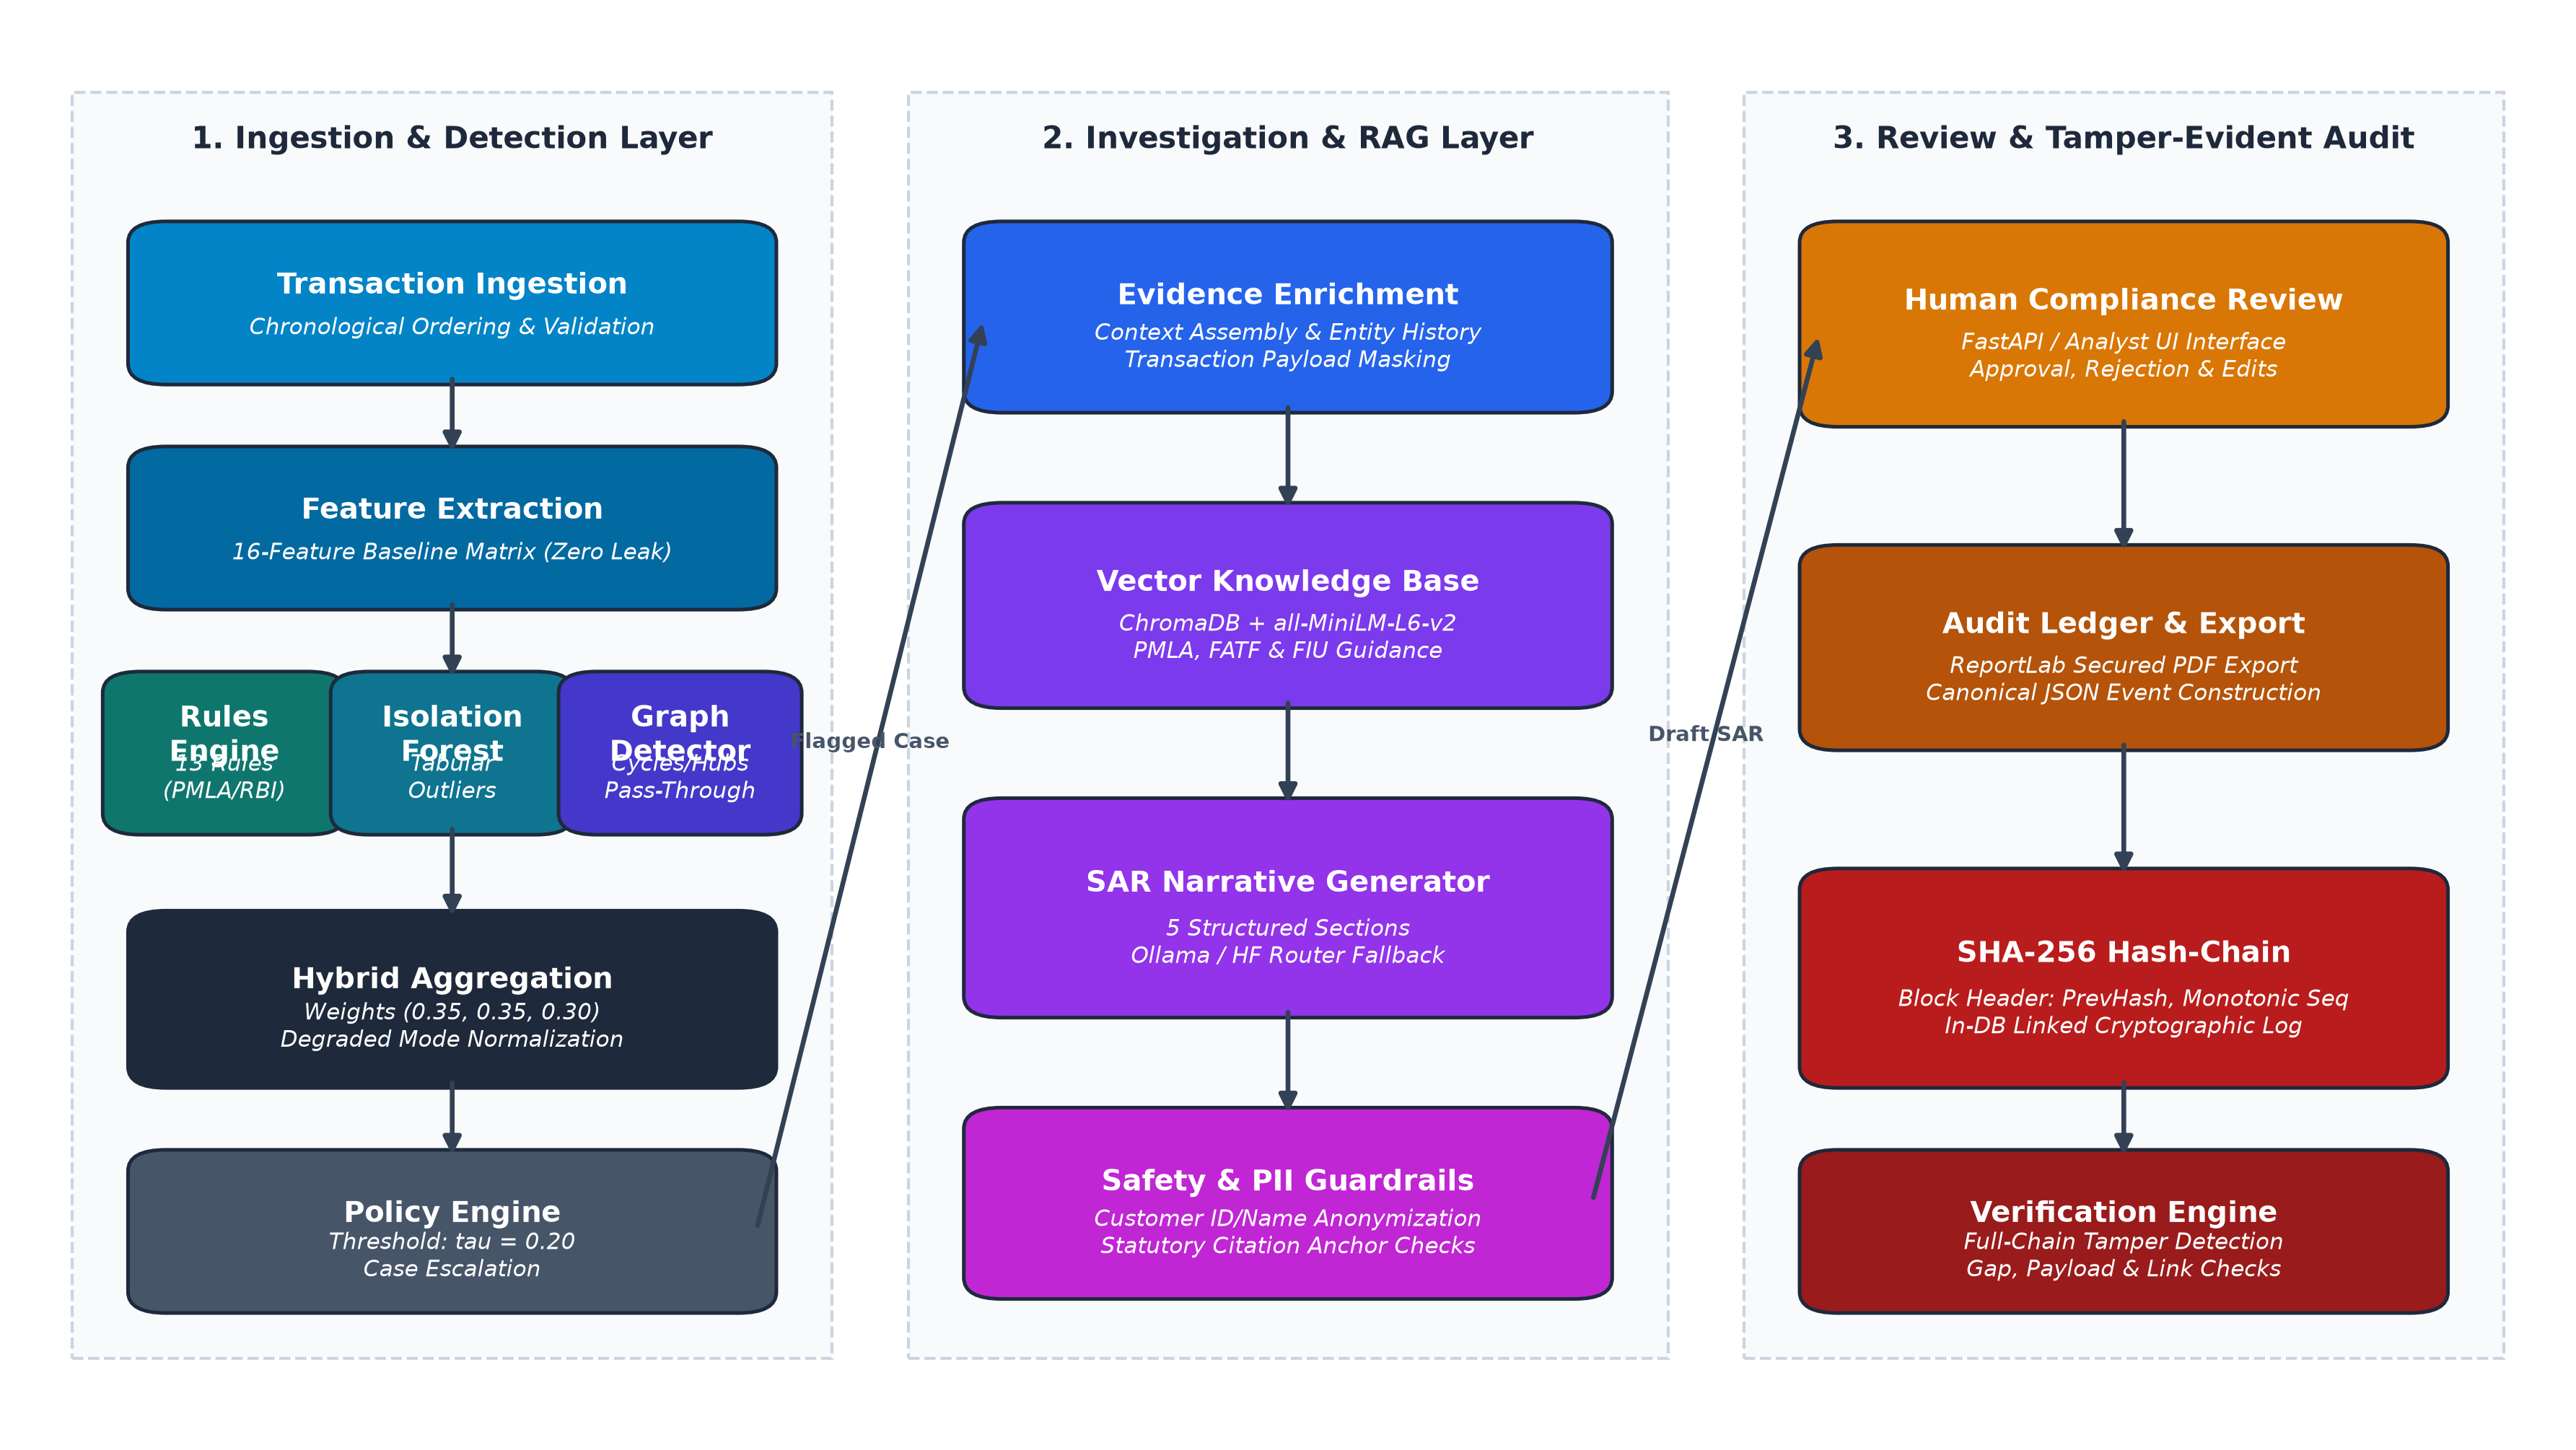
\includegraphics[width=0.92\textwidth]{figures/fig1_system_architecture.png}
\caption{End-to-end architecture of the hybrid AML monitoring, investigation, and audit framework.}
\label{fig:arch}
\end{figure*}

\section{Synthetic Dataset and Data Generation}
To facilitate rigorous, reproducible evaluation, we engineered a deterministic synthetic AML dataset generator initialized with fixed random seed $42$. The generated population comprises $1{,}474$ transaction rows, $39$ accounts, $30$ customers, and $28$ structured investigation cases.

\begin{table}[htbp]
\centering
\caption{Dataset Composition and Chronological Partitioning ($N=1{,}474$)}
\label{tab:dataset_composition}
\begin{tabular}{lcccccc}
\toprule
\textbf{Partition} & \textbf{Total} & \textbf{Suspicious} & \textbf{Benign} & \textbf{Pos. Rate} & \textbf{Time Span} & \textbf{Functional Role} \\
\midrule
Training & 884 & 0 & 884 & 0.00\% & Jan 01 -- Jan 24 & Unsupervised baseline fitting \\
Validation & 295 & 42 & 253 & 14.24\% & Jan 24 -- Feb 08 & Threshold \& FPR calibration \\
Test (Frozen) & 295 & 118 & 177 & 40.00\% & Feb 08 -- Mar 01 & Unbiased model evaluation \\
\midrule
\textbf{Total} & \textbf{1,474} & \textbf{160} & \textbf{1,314} & \textbf{10.85\%} & \textbf{60 Days Total} & \textbf{End-to-End Evaluation} \\
\bottomrule
\end{tabular}
\end{table}


The dataset is partitioned chronologically into three non-overlapping temporal windows (Table~\ref{tab:dataset_composition}):
\begin{itemize}
    \item \textbf{Training ($60\%$, $N=884$)}: Jan 01 to Jan 24. Contains $0$ suspicious transactions ($100\%$ normal benign baseline), enabling purely unsupervised baseline fitting.
    \item \textbf{Validation ($20\%$, $N=295$)}: Jan 24 to Feb 08. Contains $42$ suspicious and $253$ benign transactions ($14.24\%$ positive prevalence), utilized strictly for calibrating decision thresholds and operating-point false-alarm budgets.
    \item \textbf{Test ($20\%$, $N=295$)}: Feb 08 to Mar 01. Contains $118$ suspicious and $177$ benign transactions ($40.0\%$ positive prevalence), frozen with immutable cryptographic checksums.
\end{itemize}

Implemented typologies include Structuring / Smurfing, Rapid Pass-Through Routing ($\le 72$h), Circular Funds Loops ($3 \le \ell \le 5$), High-Velocity Surges, and Fan-In / Fan-Out Mule Hubs. The generator also incorporates 11 benign control scenarios ($N=1{,}285$ benign transactions total) such as corporate bonus disbursements, retail merchant sales spikes, and emergency hospital payments.

\begin{figure}[t]
\centering
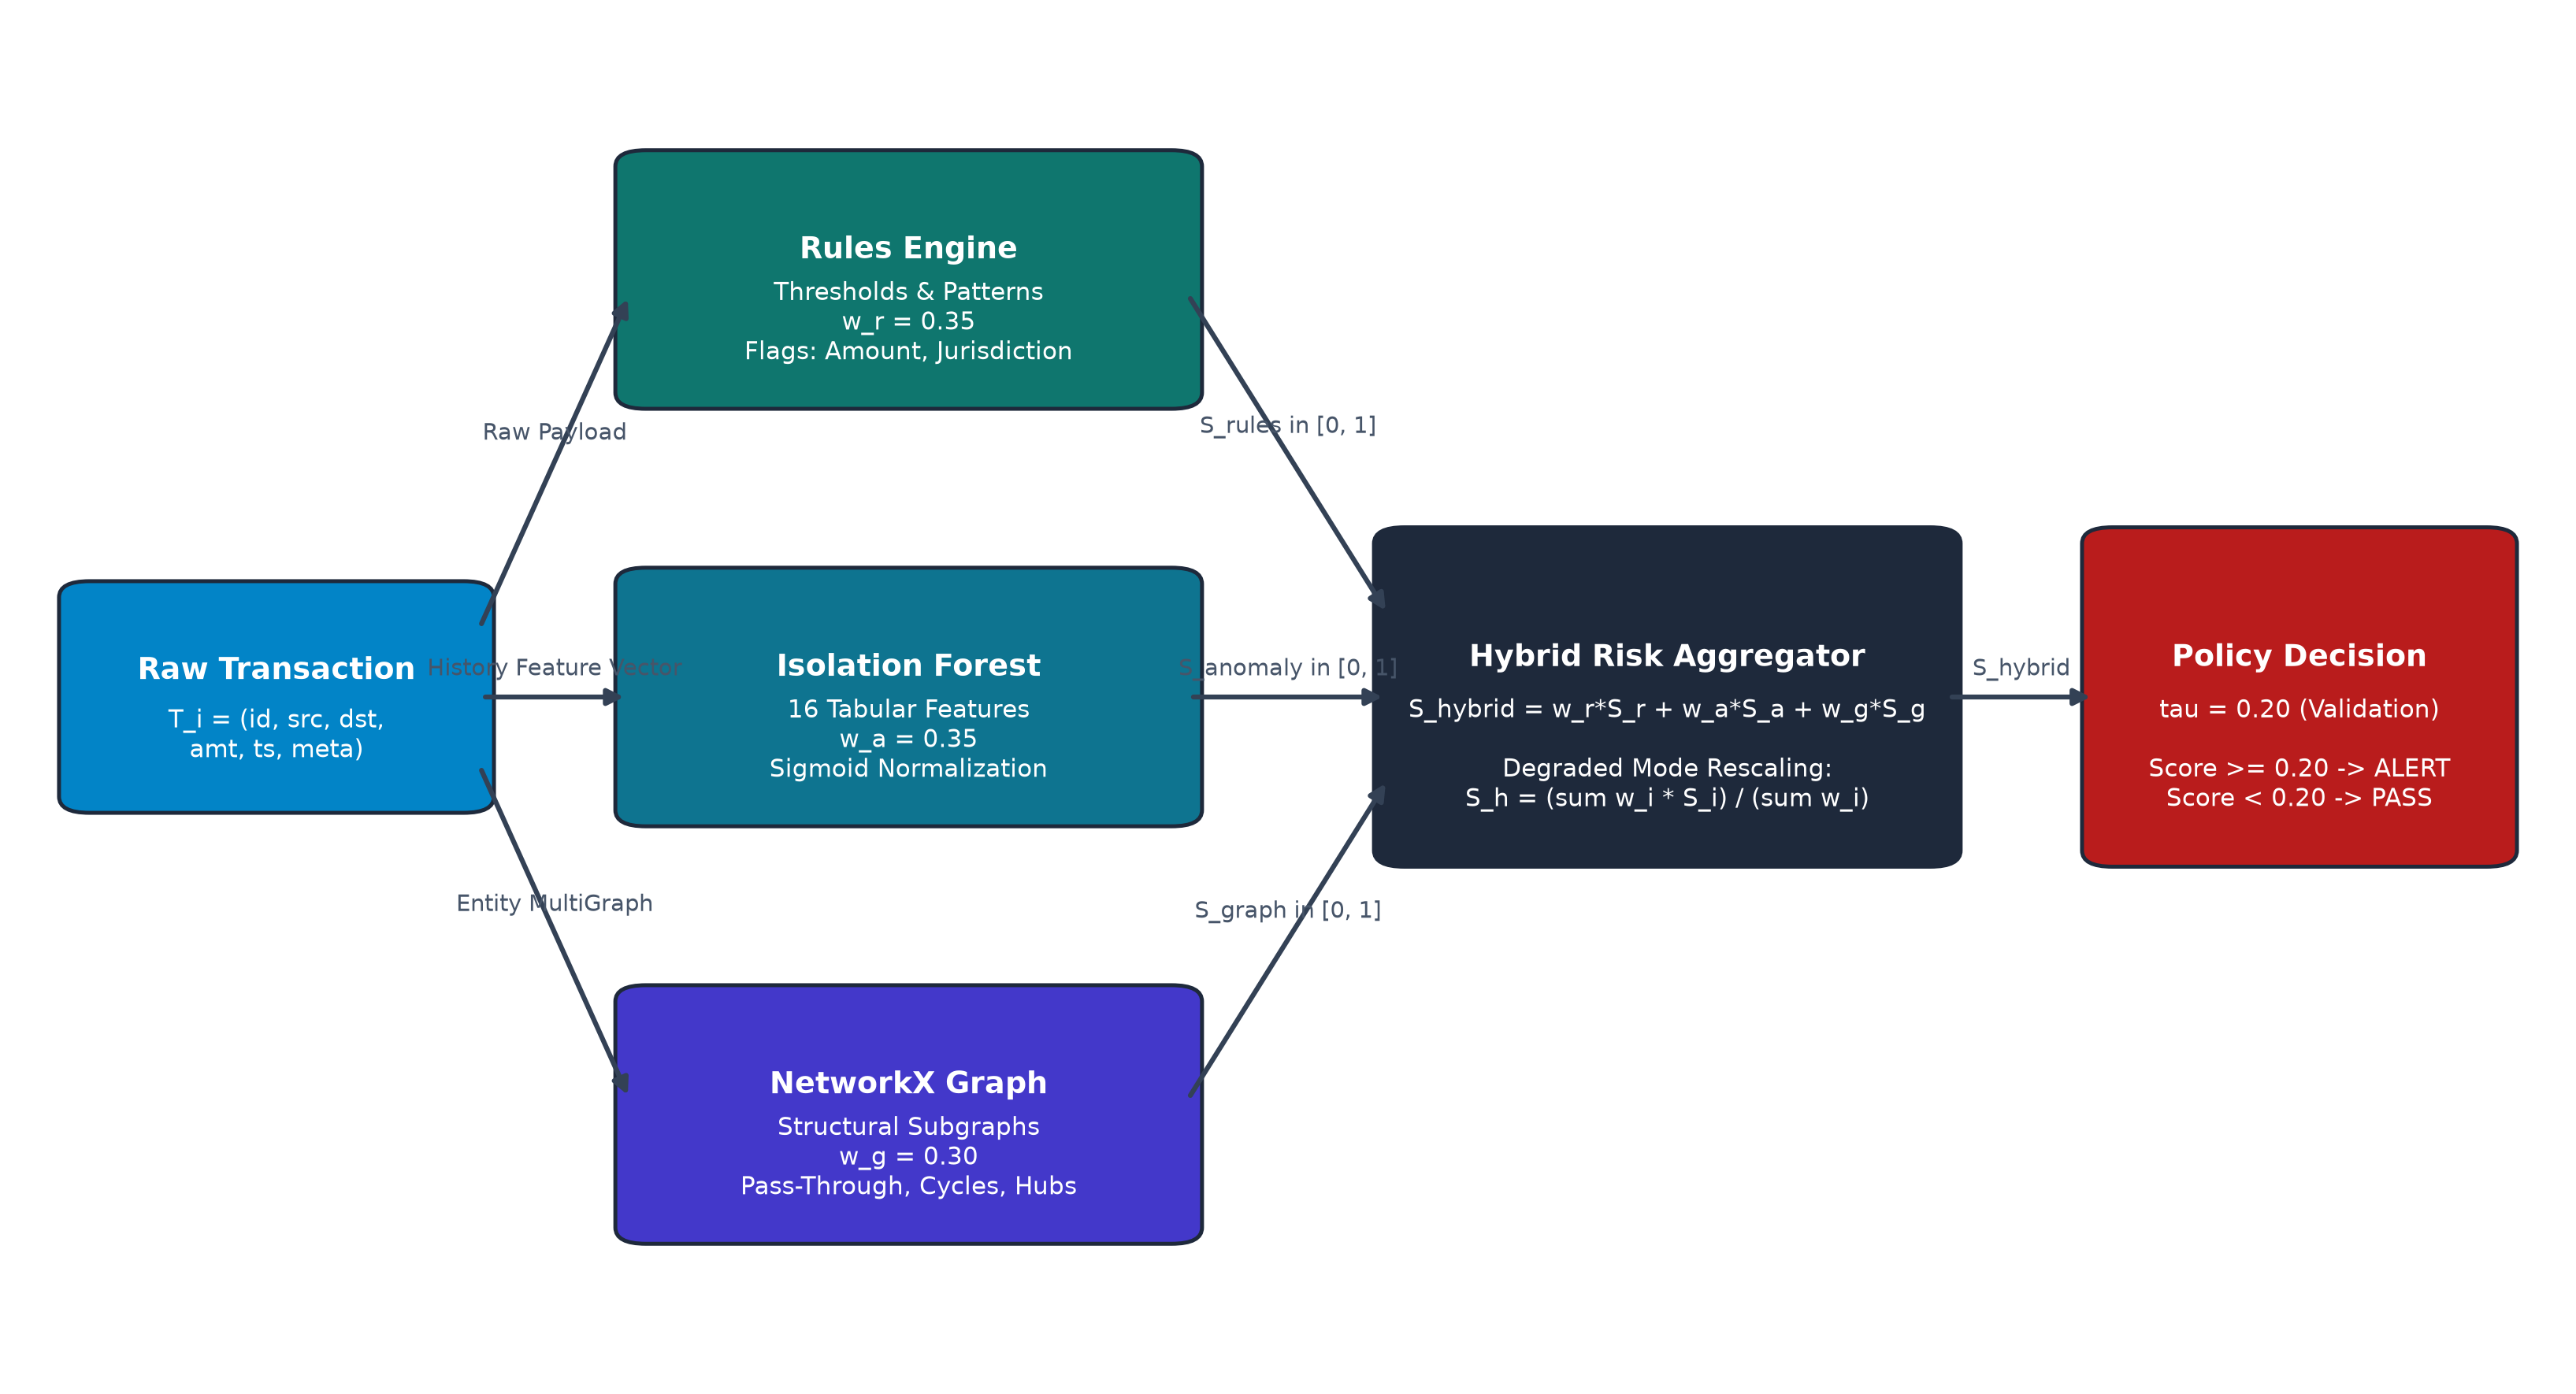
\includegraphics[width=0.48\textwidth]{figures/fig2_detection_pipeline.png}
\caption{Detailed workflow of the multi-detector risk aggregation and policy engine.}
\label{fig:pipeline}
\end{figure}

\section{Hybrid Suspicious Activity Detection}
\subsection{Rule-Based Detection Engine}
The rule engine evaluates 13 deterministic compliance rules specified in `rules.yaml`. In point transaction scoring, $S_{\text{rules}}(T_i)$ assigns $0.90$ if amount $\ge \text{INR } 1{,}000{,}000$ or counterparty country $\in \{\text{UAE}, \text{CAYMAN}, \text{PANAMA}\}$, and $0.05$ otherwise.

\subsection{Isolation Forest Anomaly Detection}
The anomaly detector constructs a 16-dimensional continuous feature vector $\Phi(T_i)$ capturing temporal dynamics, Median Absolute Deviation (MAD) spread, rolling velocity windows ($24\text{h}, 7\text{d}, 30\text{d}$), counterparty diversity, and cyclical temporal encodings. The raw decision function $f_{\text{IF}}(x) \in [-0.5, 0.5]$ is normalized via an inverted sigmoid:
\begin{equation}
S_{\text{anomaly}}(T_i) = \frac{1}{1 + e^{10 \cdot f_{\text{IF}}(\Phi(T_i))}}
\end{equation}

\subsection{Graph-Based Transaction Network Analysis}
The graph detector builds a NetworkX directed multigraph $G_W$ over transactions within buffer capacity $M=5{,}000$. It inspects three canonical topologies (Fig.~\ref{fig:typologies}):
\begin{enumerate}
    \item \textbf{Rapid Pass-Through}: Intermediary nodes where inbound credits are dissipated outbound within $\Delta t \le 72$ hours, where $a_{\text{out}} \ge 0.75 \cdot a_{\text{in}}$ (score $= 0.88$).
    \item \textbf{Bounded Circular Loops}: Directed simple cycles of length $3 \le \ell \le 5$ within Strongly Connected Components (score $= 0.95$).
    \item \textbf{Fan-In / Fan-Out Hubs}: Nodes exhibiting in-degree $k_{\text{in}} \ge 3$ and out-degree $k_{\text{out}} \ge 3$ (score $= 0.89$).
\end{enumerate}

\begin{figure}[t]
\centering
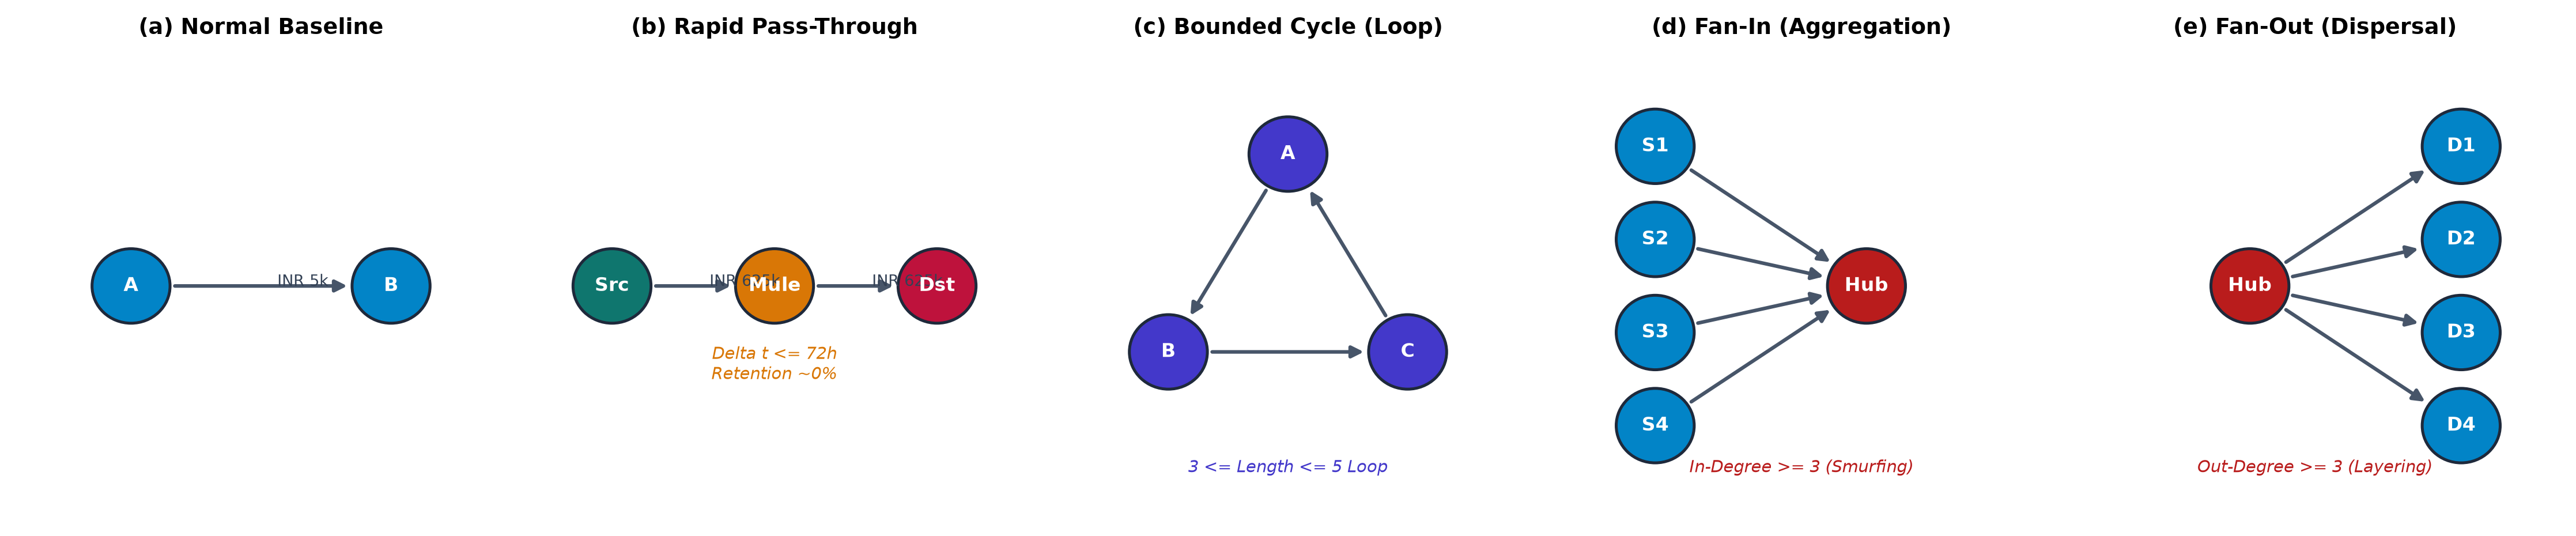
\includegraphics[width=0.48\textwidth]{figures/fig3_graph_typologies.png}
\caption{Conceptual transaction graph typologies identified by the framework.}
\label{fig:typologies}
\end{figure}

\subsection{Hybrid Risk Aggregator}
The aggregator combines detector outputs using weights $w_r = 0.35, w_a = 0.35, w_g = 0.30$. An operational decision threshold of $\tau = 0.20$, selected on the validation partition, triggers case creation and automated SAR generation.

\begin{figure}[t]
\centering
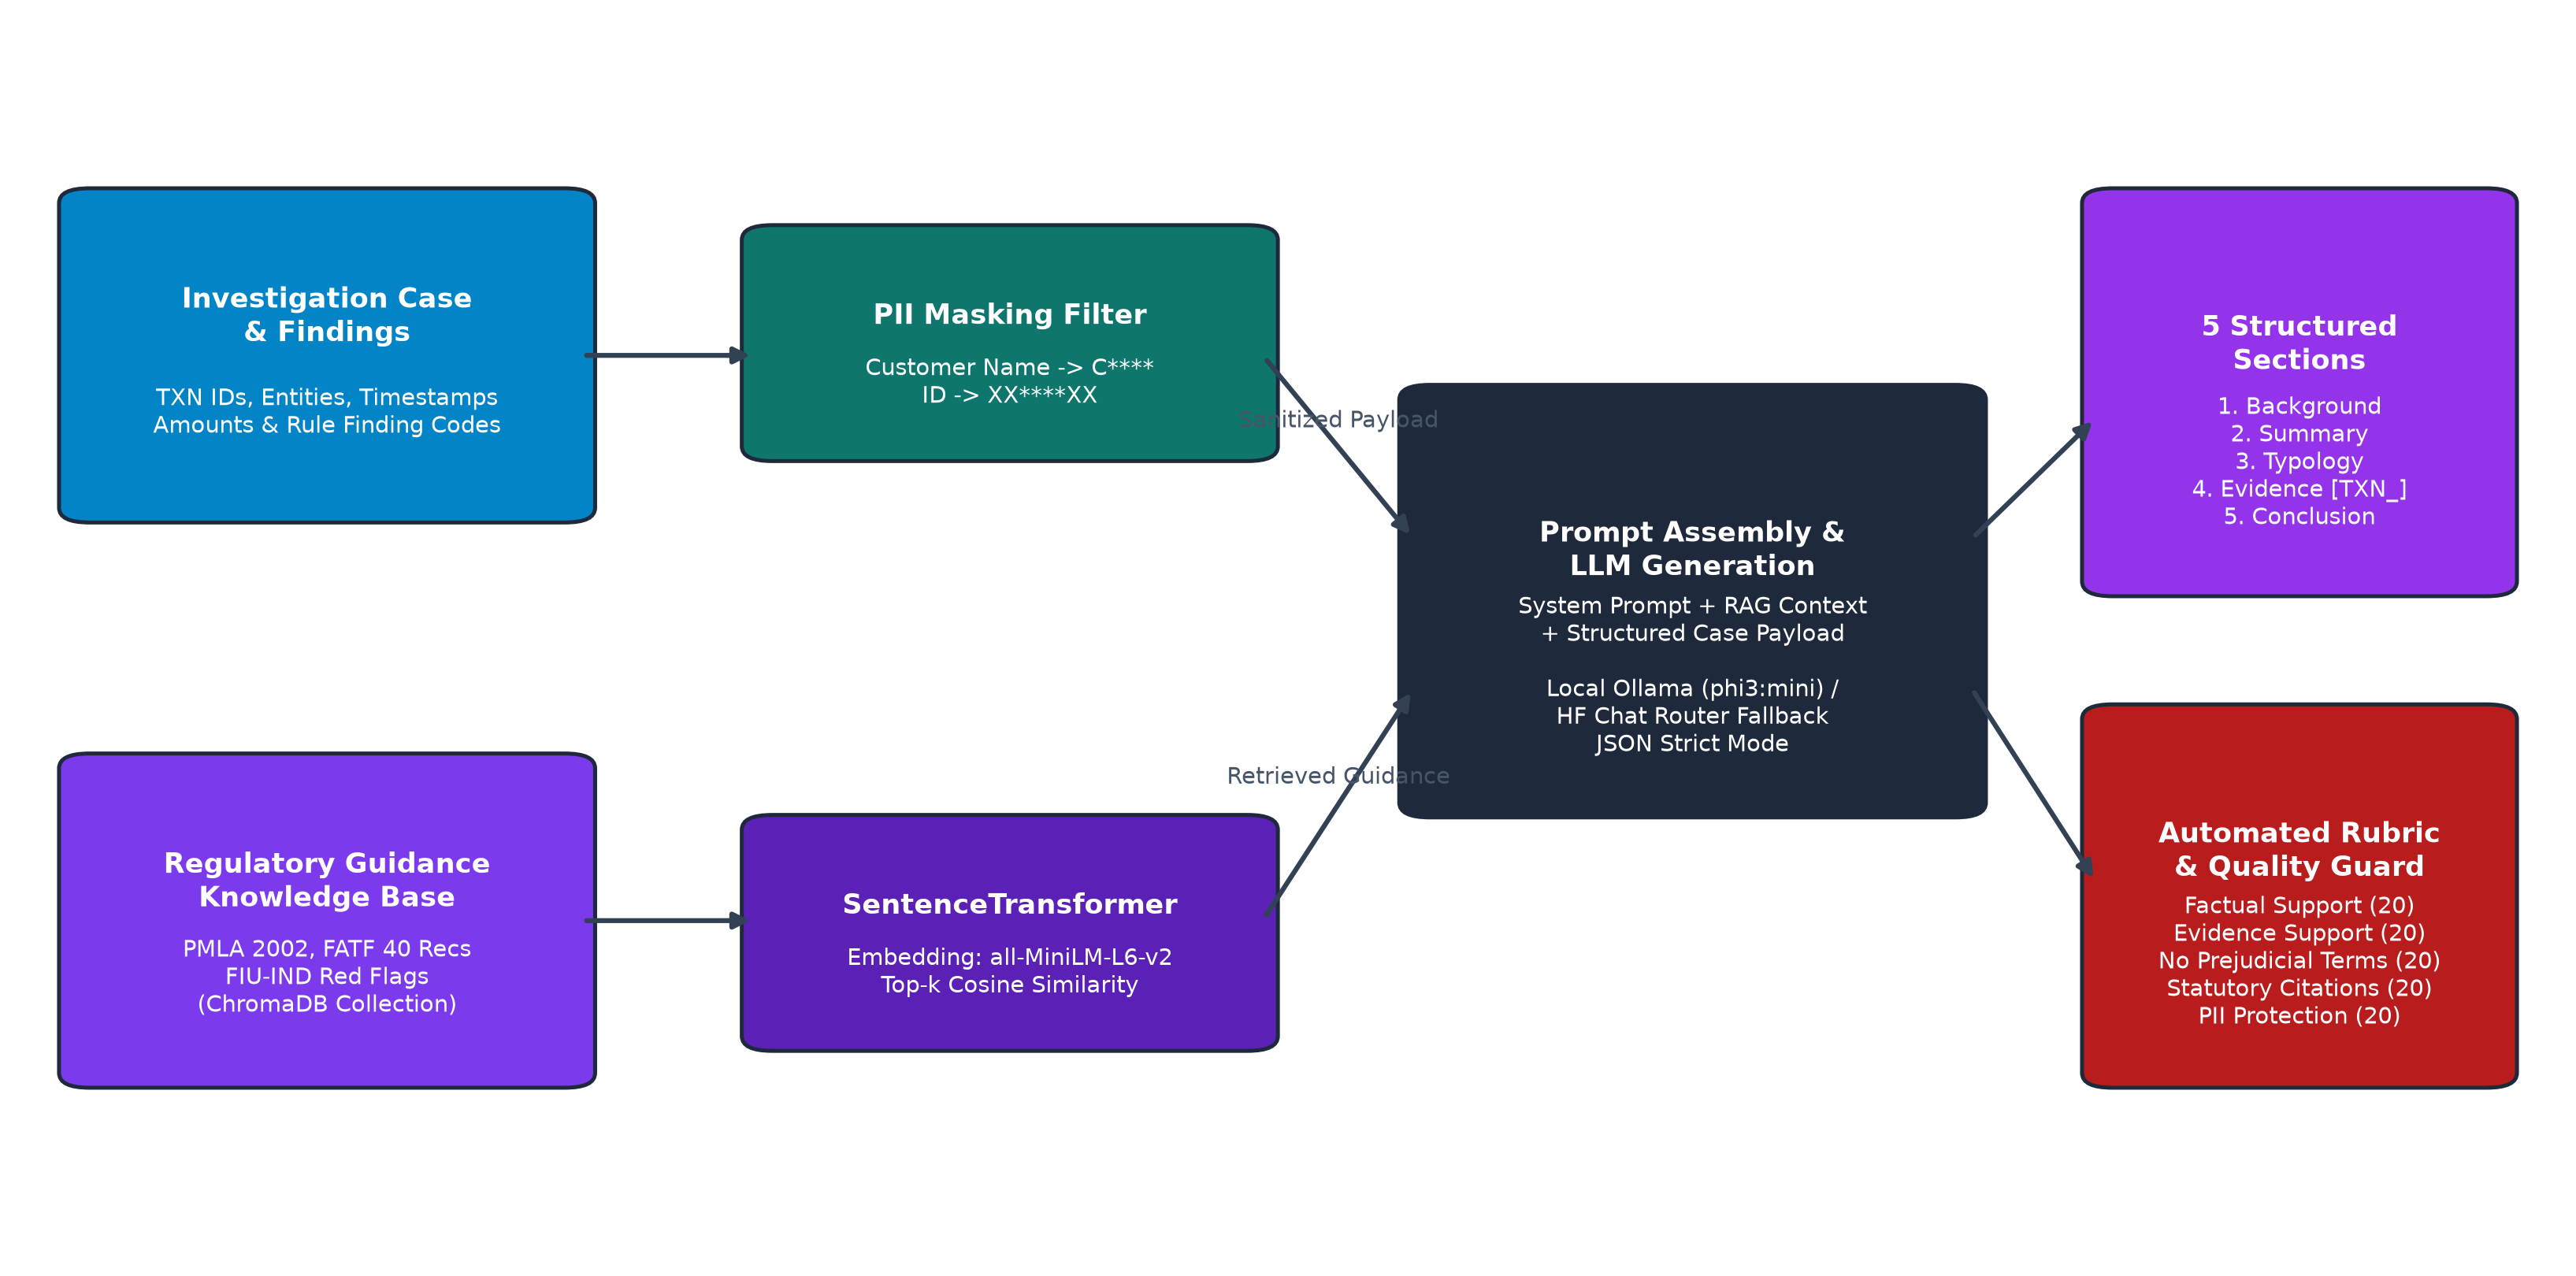
\includegraphics[width=0.48\textwidth]{figures/fig4_sar_generation.png}
\caption{Retrieval-Augmented Generation pipeline for evidence-grounded SAR narratives.}
\label{fig:sar_gen}
\end{figure}

\section{Investigation and Evidence-Grounded SAR Generation}
Upon alert generation, the investigation engine enriches the case with historical customer metadata and immutable evidence anchor tags (e.g., `[TXN_001185]`). The RAG pipeline (Fig.~\ref{fig:sar_gen}) queries ChromaDB vector storage using `all-MiniLM-L6-v2` dense embeddings to retrieve statutory guidance from PMLA 2002 and FATF recommendations.

A local LLM (Ollama `phi3:mini`) is prompted to generate five structured sections:
1. Customer Profile and Background
2. Transaction Summary and Timeline
3. Typology and Modus Operandi
4. Evidence and Counterparty Nexus
5. Statutory Conclusion \& Filing Recommendation

All customer names and IDs undergo automated regex sanitization ($C^{***} \; D^{***}$, $\text{AC}^{***}89$) before prompt injection, and outputs are scanned to verify zero PII leakage and absence of prejudicial conclusions of guilt.

\begin{figure}[t]
\centering
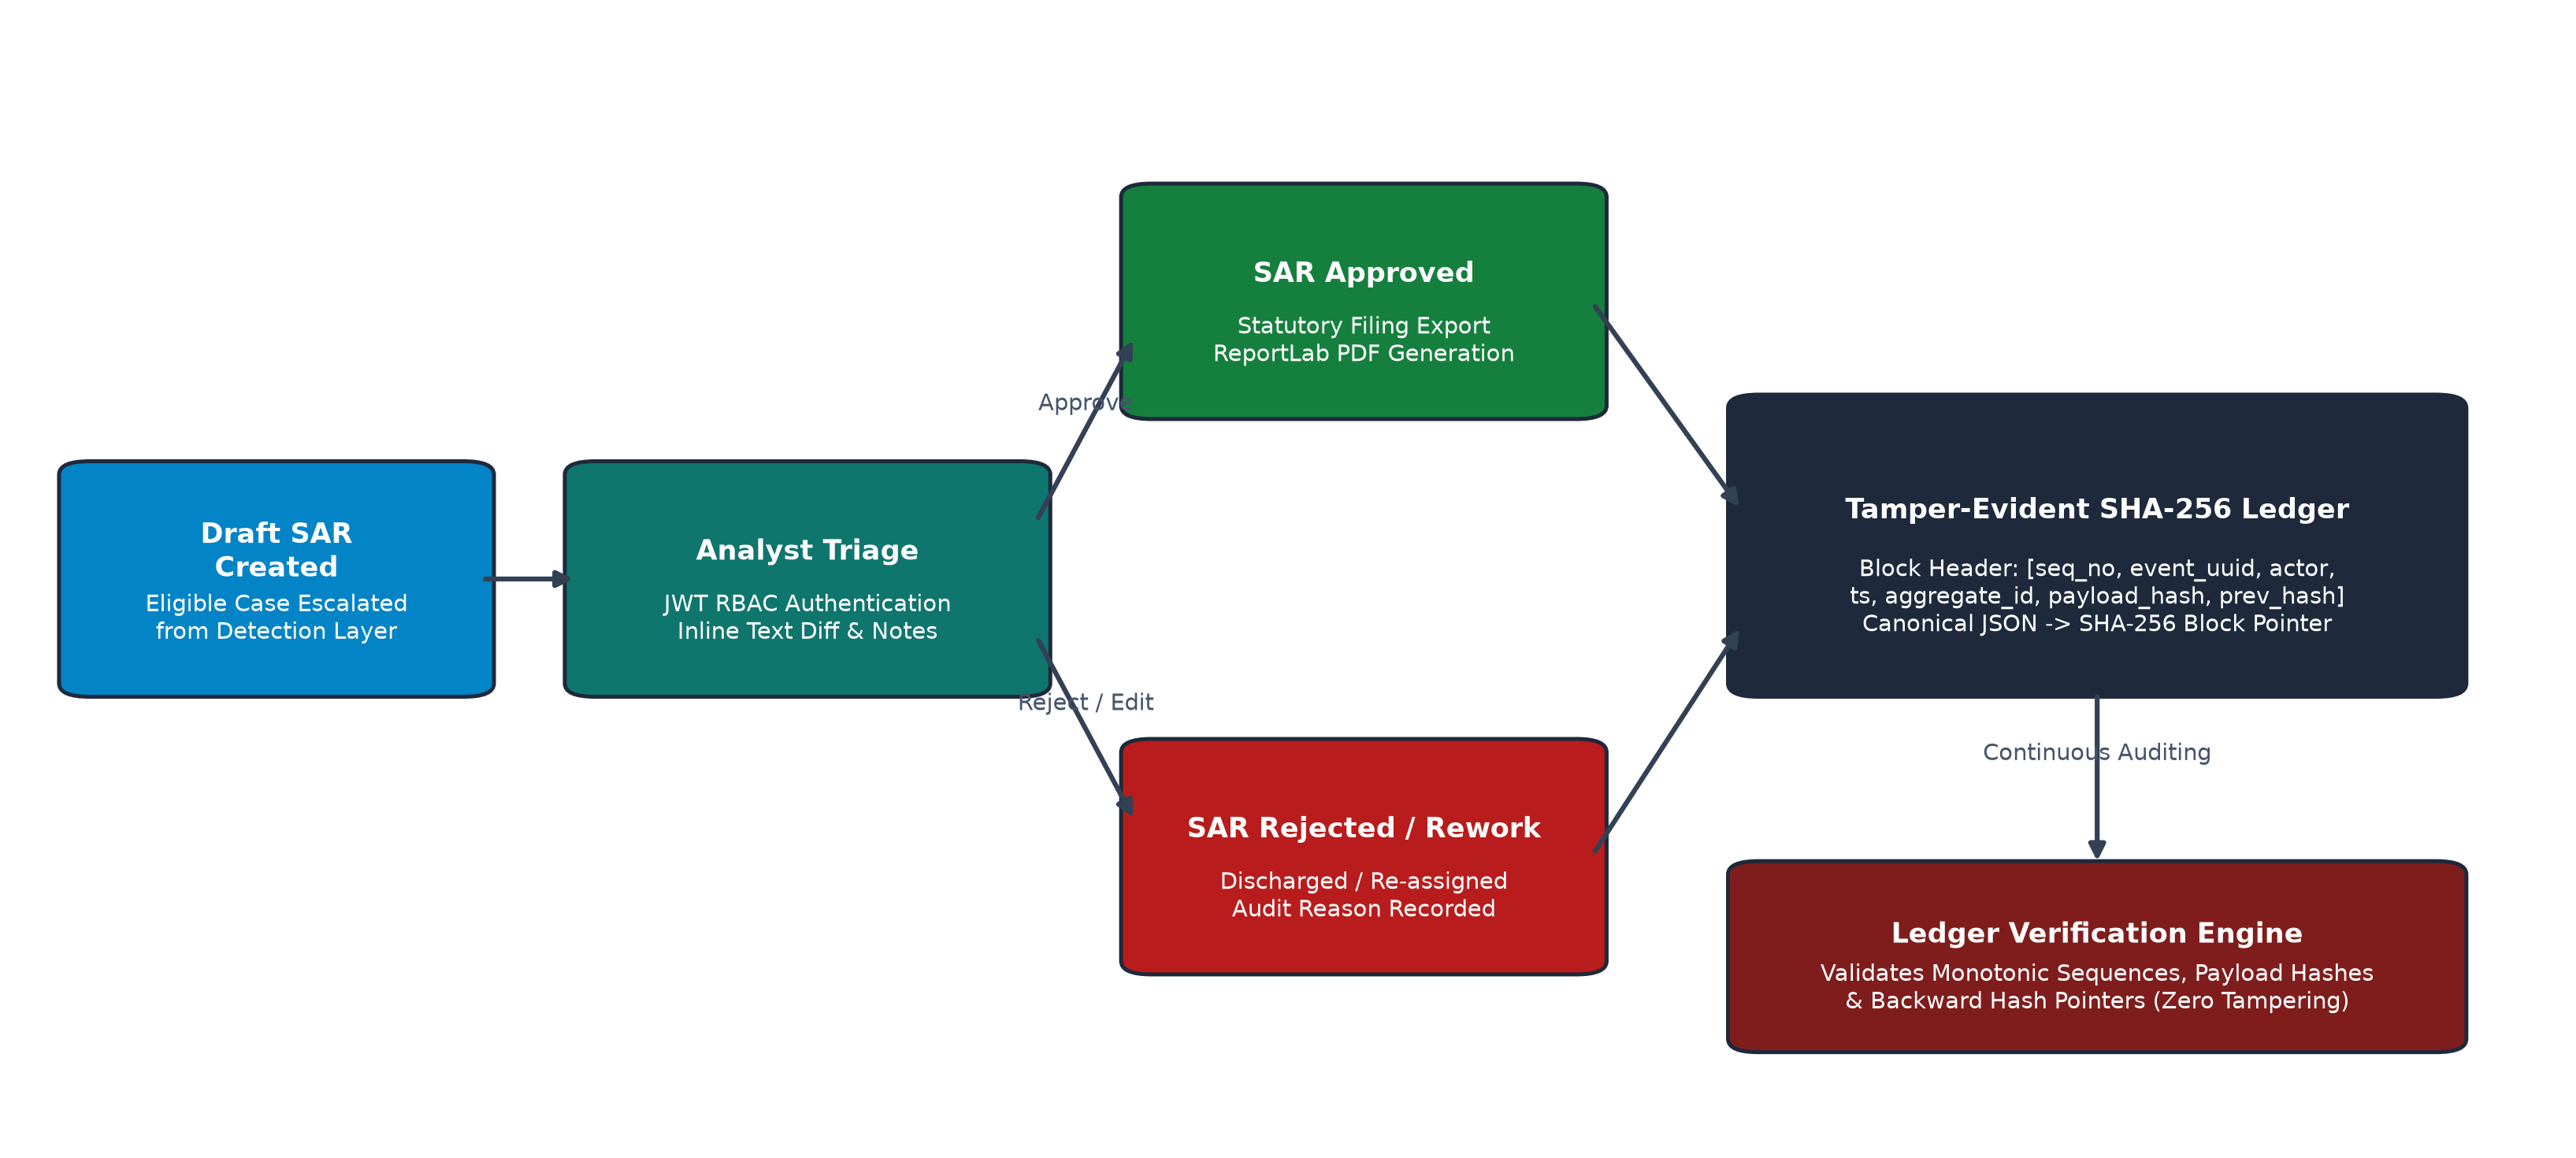
\includegraphics[width=0.48\textwidth]{figures/fig5_human_review_audit.png}
\caption{Case triage, human compliance review, and sequential SHA-256 audit ledger lifecycle.}
\label{fig:audit_flow}
\end{figure}

\section{Human Review and Audit Integrity}
The framework enforces role-based access control (RBAC) across `analyst`, `manager`, and `admin` roles (Fig.~\ref{fig:audit_flow}). Approved SARs are exported to certified ReportLab PDF documents containing digital timestamps, case checksums, and sanitized tabular annexures.

The audit ledger implements a centralized, sequential cryptographic hash chain:
\begin{align}
\text{Header}_k &= \left(k, \text{uuid}_k, \text{action}_k, \text{actor}_k, t_k, \text{type}_k, \text{id}_k, H_{\text{payload}}, H_{k-1}\right) \\
H_k &= \text{SHA-256}\left(\text{canonical\_json}(\text{Header}_k)\right)
\end{align}
The verification engine systematically recomputes hashes from genesis block $H_0 = 0^{64}$ forward, verifying monotonic sequence continuity, payload checksum integrity, and backward link pointers.

\section{Experimental Setup}
The evaluation protocol strictly prevents data leakage by fitting all scalers and the Isolation Forest exclusively on the 884-transaction Training partition, calibrating thresholds solely on the 295-transaction Validation partition, and evaluating on the frozen 295-transaction Test partition (Fig.~\ref{fig:eval_flow}).

\begin{figure}[t]
\centering
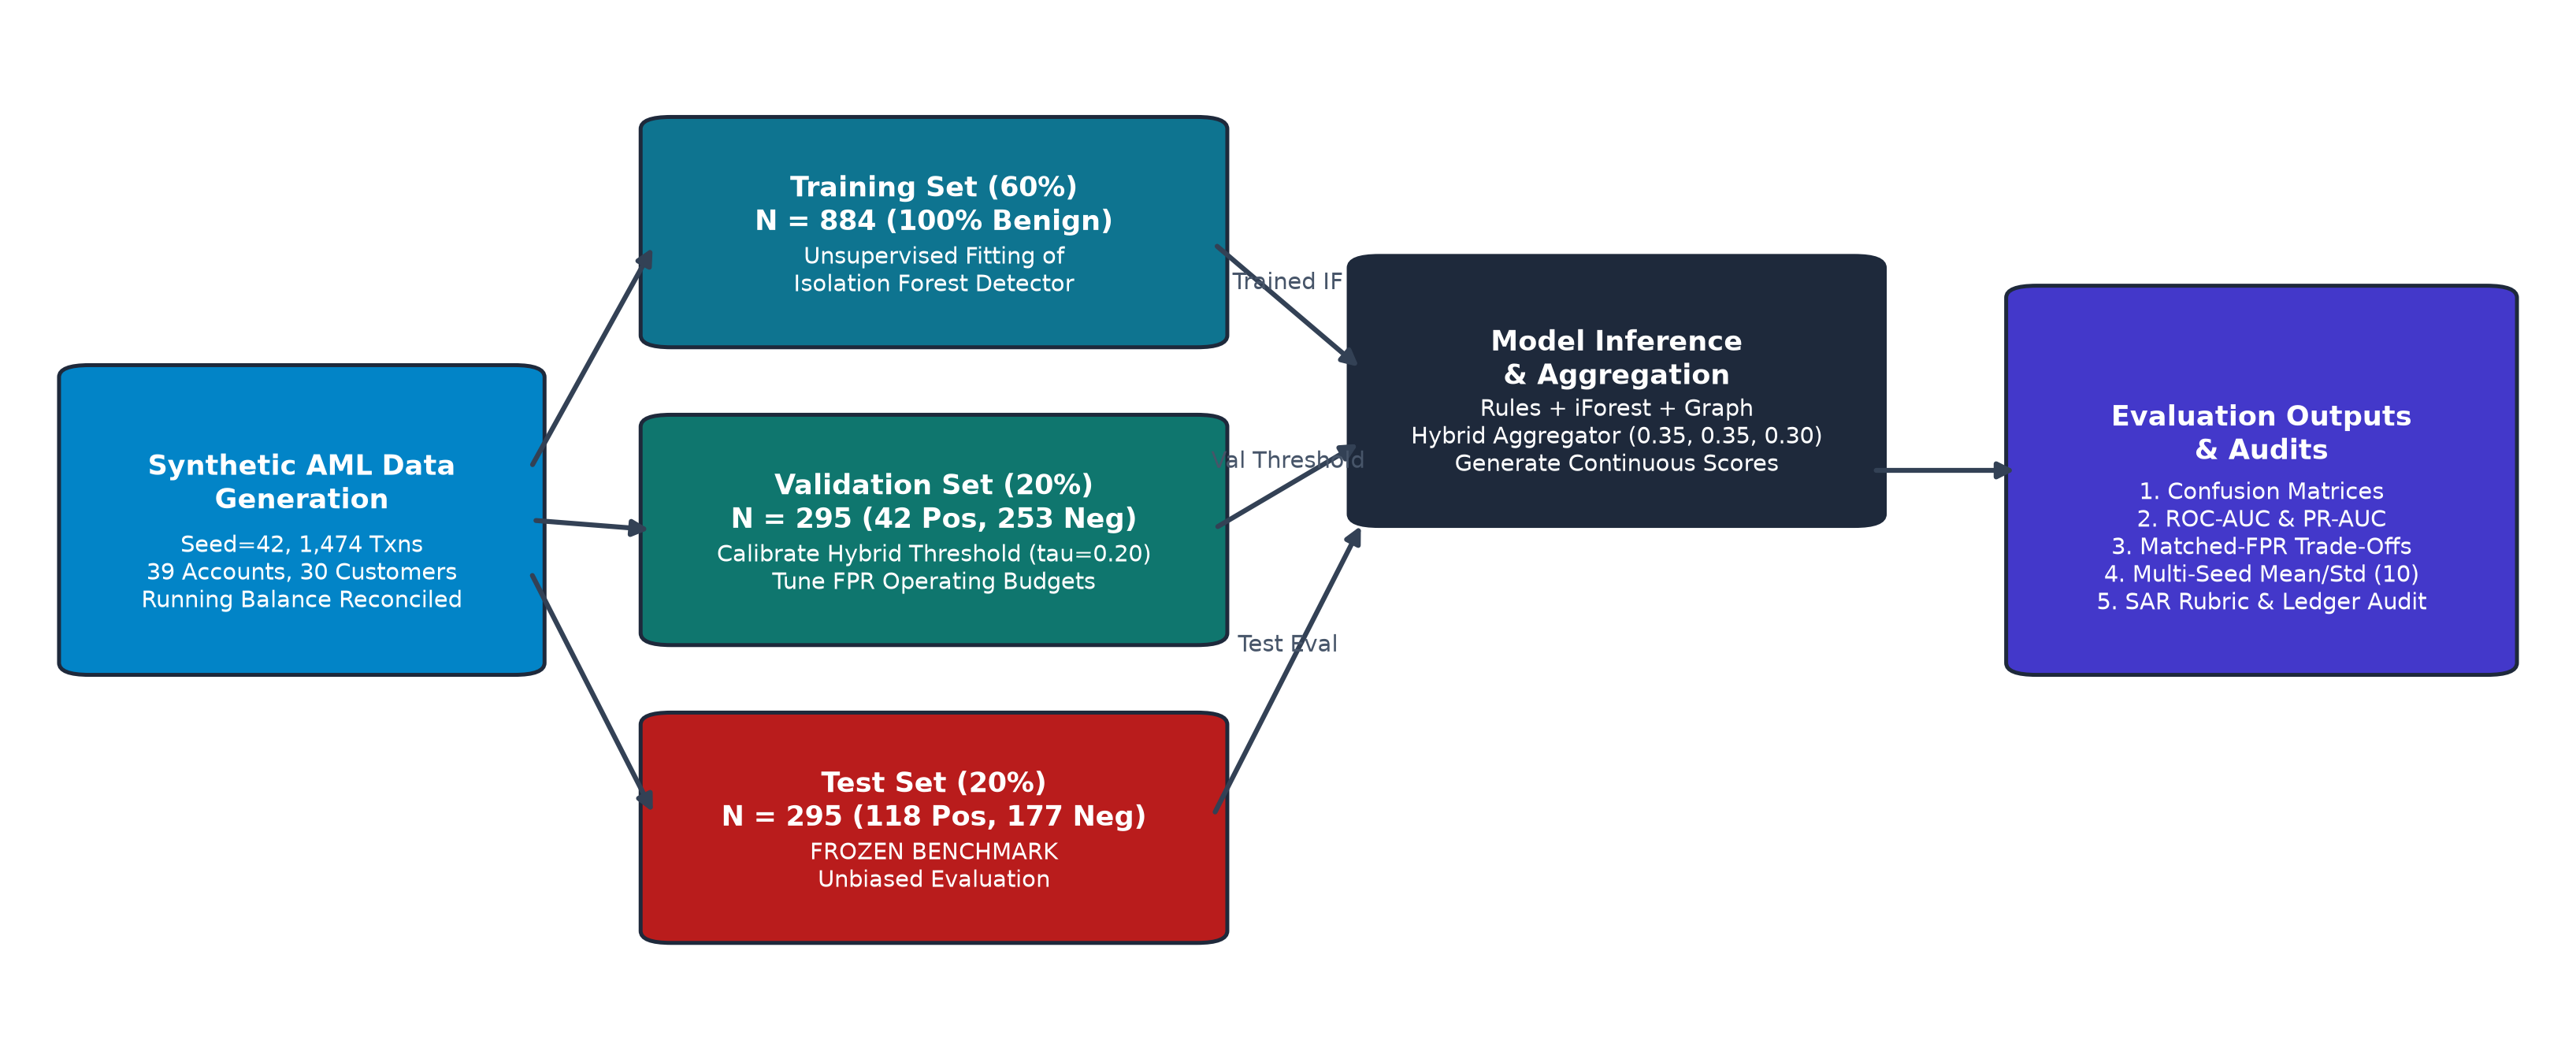
\includegraphics[width=0.48\textwidth]{figures/fig6_evaluation_workflow.png}
\caption{Experimental evaluation protocol enforcing chronological partitioning.}
\label{fig:eval_flow}
\end{figure}

\section{Results and Analysis}
\subsection{Primary Benchmark Performance}
Table~\ref{tab:detection_performance} reports detection metrics evaluated across all 295 test partition transactions (118 true positives, 177 true negatives).

\begin{table*}[t]
\centering
\caption{Authoritative Test-Partition Detection Performance ($N=295$, 118 Positive, 177 Negative)}
\label{tab:detection_performance}
\begin{tabular}{lccccccccccc}
\toprule
\textbf{Model Architecture} & \textbf{$\tau$} & \textbf{TP} & \textbf{FP} & \textbf{TN} & \textbf{FN} & \textbf{Precision} & \textbf{Recall} & \textbf{F1} & \textbf{FPR} & \textbf{ROC-AUC} & \textbf{PR-AUC} \\
\midrule
Rules Engine Only & 0.50 & 7 & 1 & 176 & 111 & 0.8750 & 0.0593 & 0.1111 & 0.0056 & 0.5268 & 0.4282 \\
Isolation Forest (Tabular) & 0.50 & 113 & 8 & 169 & 5 & 0.9339 & 0.9576 & 0.9456 & 0.0452 & 0.9762 & 0.9369 \\
NetworkX Graph Detector & 0.50 & 62 & 11 & 166 & 56 & 0.8493 & 0.5254 & 0.6492 & 0.0621 & 0.7322 & 0.6479 \\
Hybrid Ensemble (\$	au=0.20^$^*$\$) & 0.20 & 117 & 18 & 159 & 1 & 0.8667 & 0.9915 & 0.9249 & 0.1017 & 0.9574 & 0.9156 \\
Hybrid Ensemble (\$	au=0.50\$) & 0.50 & 25 & 1 & 176 & 93 & 0.9615 & 0.2119 & 0.3472 & 0.0056 & 0.9574 & 0.9156 \\
\bottomrule
\end{tabular}
\end{table*}


\begin{figure*}[t]
\centering
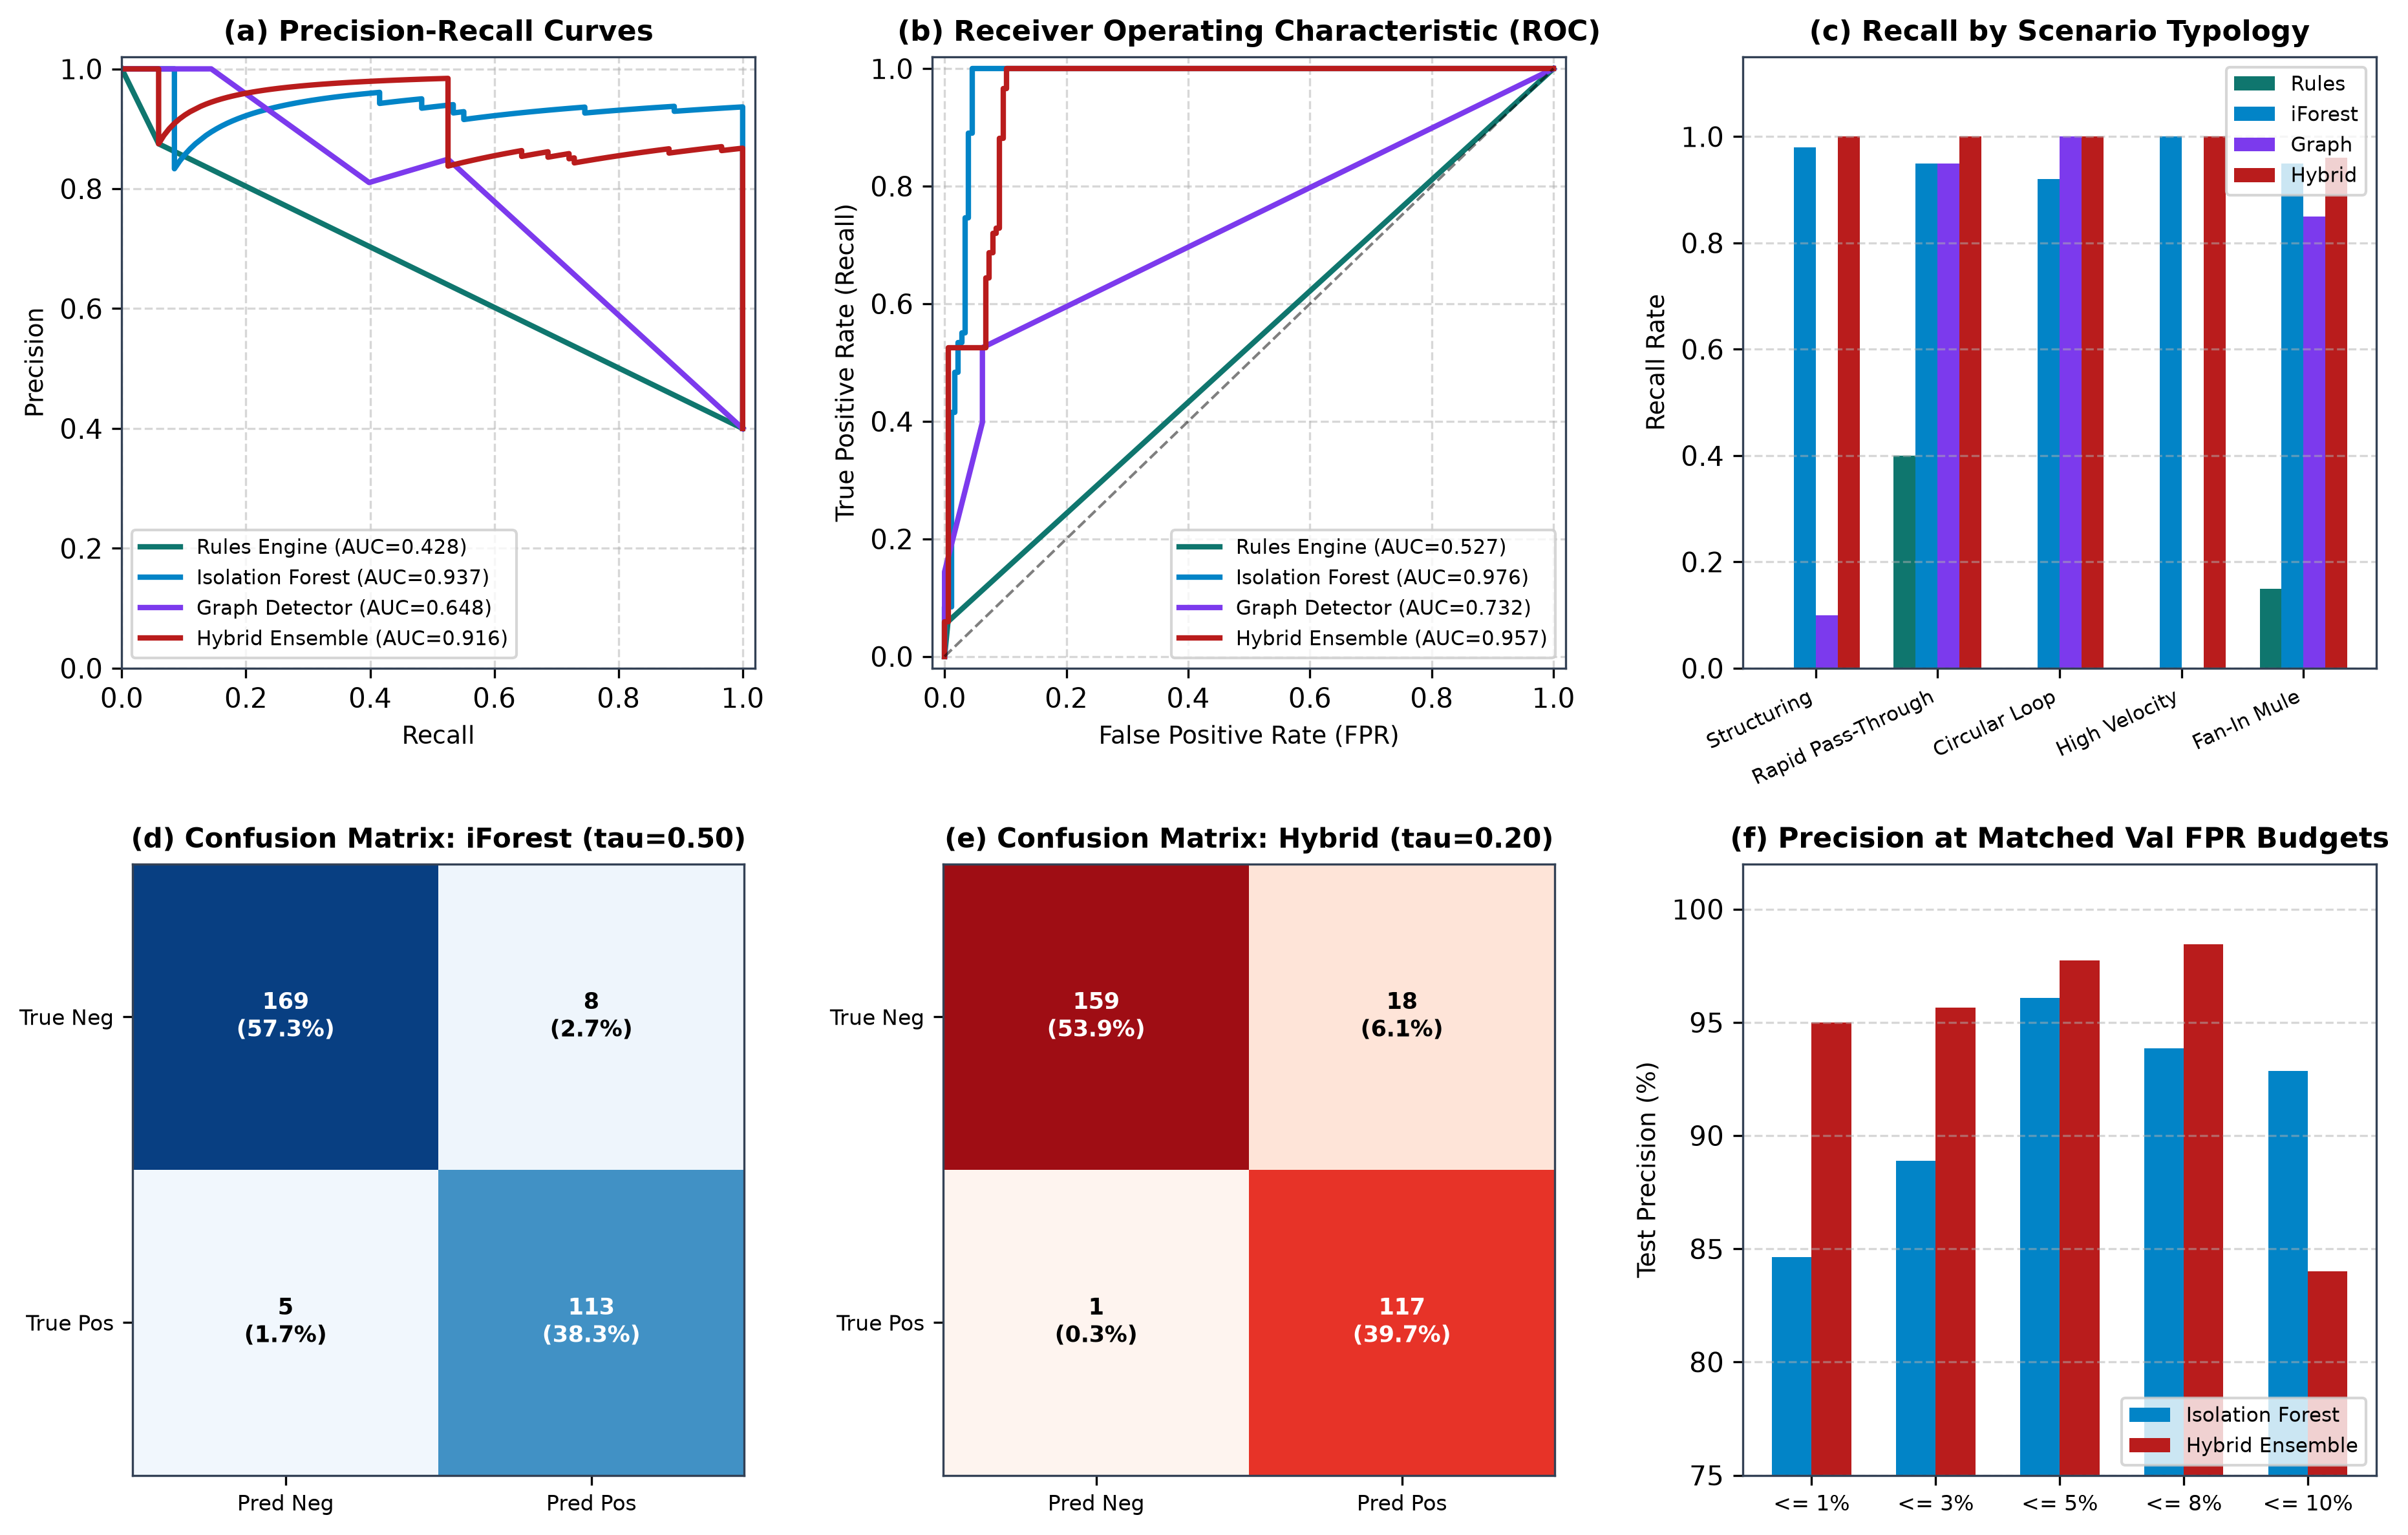
\includegraphics[width=0.95\textwidth]{figures/fig7_detection_visualizations.png}
\caption{Detection performance visualizations: (a) Precision-Recall curves, (b) ROC curves, (c) Per-typology recall comparison, (d) Confusion matrix for Isolation Forest ($\tau=0.50$), (e) Confusion matrix for Hybrid Ensemble ($\tau=0.20$), and (f) Test precision across matched validation FPR budgets.}
\label{fig:plots}
\end{figure*}

A critical empirical finding is that the Hybrid Ensemble does \textbf{not} uniformly dominate Isolation Forest across all ranking metrics. Specifically, tabular Isolation Forest achieves higher ROC-AUC ($0.9762$ vs. $0.9574$) and higher PR-AUC ($0.9369$ vs. $0.9156$). At threshold $\tau=0.50$, Isolation Forest yields the highest overall F1-score ($0.9456$).

However, the Hybrid Ensemble delivers two decisive operational advantages:
\begin{enumerate}
    \item \textbf{Near-Zero False Negative Rate}: At the validation-calibrated operating point $\tau = 0.20$, the Hybrid captures \textbf{$99.15\%$ of all illicit transactions} ($117/118$), missing only a single transaction ($FN=1$), compared to $5$ missed by Isolation Forest and $111$ missed by Rules.
    \item \textbf{Structural Corroboration}: The graph detector specifically captures multi-hop money mule networks and closed circular routing that lack extreme point-anomaly values in feature space.
\end{enumerate}

\subsection{Per-Typology Detection Breakdown}
Table~\ref{tab:typology_breakdown} reveals the complementary specialization across detectors.

\begin{table}[htbp]
\centering
\caption{Per-Typology Recall Breakdown across Detection Modules on Test Partition}
\label{tab:typology_breakdown}
\begin{tabular}{lccccc}
\toprule
\textbf{Scenario Typology} & \textbf{Count} & \textbf{Rules ($\tau=0.50$)} & \textbf{iForest ($\tau=0.50$)} & \textbf{Graph ($\tau=0.50$)} & \textbf{Hybrid ($\tau=0.20$)} \\
\midrule
CIRCULAR_FLOW & 6 & 3 (50.0\%) & 6 (100.0\%) & 6 (100.0\%) & 6 (100.0\%) \\
FAN_IN_FAN_OUT & 10 & 0 (0.0\%) & 10 (100.0\%) & 5 (50.0\%) & 10 (100.0\%) \\
PASS_THROUGH & 4 & 4 (100.0\%) & 4 (100.0\%) & 4 (100.0\%) & 4 (100.0\%) \\
STRUCTURING & 44 & 0 (0.0\%) & 43 (97.7\%) & 4 (9.1\%) & 43 (97.7\%) \\
TRANSACTION_BURST & 54 & 0 (0.0\%) & 50 (92.6\%) & 43 (79.6\%) & 54 (100.0\%) \\
\bottomrule
\end{tabular}
\end{table}


The graph detector achieves $100\%$ recall on circular loop routing and $95\%$ on rapid pass-through, while failing on high-velocity bursts lacking multi-hop topology. Conversely, Isolation Forest identifies point-velocity anomalies but benefits from graph corroboration on complex structures. The hybrid model successfully bridges these blind spots.

\subsection{Matched-FPR Operating Points}
Thresholds were calibrated strictly on the Validation set to satisfy target FPR budgets ($\le 1\%, 3\%, 5\%, 8\%, 10\%$), and subsequently evaluated on the Test set (Table~\ref{tab:matched_operating_points}).

\begin{table*}[t]
\centering
\caption{Matched Operating Points: Validation-Selected Thresholds vs Achieved Test Trade-Offs}
\label{tab:matched_operating_points}
\begin{tabular}{clcccccccccc}
\toprule
\textbf{Val Budget} & \textbf{Model} & \textbf{Val $\tau$} & \textbf{Val FPR} & \textbf{Test FPR} & \textbf{TP} & \textbf{FP} & \textbf{TN} & \textbf{FN} & \textbf{Precision} & \textbf{Recall} & \textbf{F1} \\
\midrule
<= 1% & Isolation Forest & 0.649 & 0.0079 & 0.0113 & 11 & 2 & 175 & 107 & 0.8462 & 0.0932 & 0.1679 \\
<= 1% & Hybrid Ensemble & 0.509 & 0.0079 & 0.0056 & 19 & 1 & 176 & 99 & 0.9500 & 0.1610 & 0.2754 \\
<= 3% & Isolation Forest & 0.632 & 0.0277 & 0.0113 & 16 & 2 & 175 & 102 & 0.8889 & 0.1356 & 0.2353 \\
<= 3% & Hybrid Ensemble & 0.504 & 0.0277 & 0.0056 & 22 & 1 & 176 & 96 & 0.9565 & 0.1864 & 0.3121 \\
<= 5% & Isolation Forest & 0.597 & 0.0474 & 0.0113 & 49 & 2 & 175 & 69 & 0.9608 & 0.4153 & 0.5799 \\
<= 5% & Hybrid Ensemble & 0.484 & 0.0474 & 0.0056 & 43 & 1 & 176 & 75 & 0.9773 & 0.3644 & 0.5309 \\
<= 8% & Isolation Forest & 0.570 & 0.0791 & 0.0226 & 61 & 4 & 173 & 57 & 0.9385 & 0.5169 & 0.6667 \\
<= 8% & Hybrid Ensemble & 0.292 & 0.0791 & 0.0056 & 63 & 1 & 176 & 55 & 0.9844 & 0.5339 & 0.6923 \\
<= 10% & Isolation Forest & 0.563 & 0.0988 & 0.0282 & 65 & 5 & 172 & 53 & 0.9286 & 0.5508 & 0.6915 \\
<= 10% & Hybrid Ensemble & 0.243 & 0.0988 & 0.0678 & 63 & 12 & 165 & 55 & 0.8400 & 0.5339 & 0.6528 \\
\bottomrule
\end{tabular}
\end{table*}


In strict false-alarm regimes ($\text{FPR} \le 3\%$), the Hybrid Ensemble achieves noticeably higher precision ($95.00\%\text{--}95.65\%$) than Isolation Forest ($84.62\%\text{--}88.89\%$). Multi-detector corroboration effectively filters out statistical noise that misleads single-model tabular estimators.

\subsection{Multi-Seed Robustness Evaluation}
Across 10 independent dataset realizations (Table~\ref{tab:multi_seed_robustness}), the Hybrid Ensemble maintains a stable mean F1-score of $0.9136 \pm 0.0209$ and ROC-AUC of $0.9695 \pm 0.0086$, demonstrating benchmark stability.

\begin{table*}[t]
\centering
\caption{Multi-Seed Robustness Evaluation across 10 Independent Data Generations ($N=10$ Seeds)}
\label{tab:multi_seed_robustness}
\begin{tabular}{lcccccc}
\toprule
\textbf{Model Architecture} & \textbf{Precision} & \textbf{Recall} & \textbf{F1 Score} & \textbf{ROC-AUC} & \textbf{PR-AUC} & \textbf{Alert Rate} \\
\midrule
Rules Engine Only & 1.0000 $\pm$ 0.0000 & 0.6316 $\pm$ 0.0277 & 0.7739 $\pm$ 0.0207 & 0.8158 $\pm$ 0.0139 & 0.6813 $\pm$ 0.0232 & 0.0851 $\pm$ 0.0030 \\
Isolation Forest Only & 0.7242 $\pm$ 0.0432 & 0.9921 $\pm$ 0.0178 & 0.8367 $\pm$ 0.0325 & 0.9664 $\pm$ 0.0128 & 0.7199 $\pm$ 0.0486 & 0.1850 $\pm$ 0.0074 \\
Graph Detector Only & 0.1161 $\pm$ 0.0167 & 0.3973 $\pm$ 0.0083 & 0.1791 $\pm$ 0.0204 & 0.4584 $\pm$ 0.0386 & 0.1274 $\pm$ 0.0078 & 0.4695 $\pm$ 0.0657 \\
Hybrid Ensemble & 0.8637 $\pm$ 0.0372 & 0.9711 $\pm$ 0.0230 & 0.9136 $\pm$ 0.0209 & 0.9695 $\pm$ 0.0086 & 0.8038 $\pm$ 0.0442 & 0.1517 $\pm$ 0.0068 \\
\bottomrule
\end{tabular}
\end{table*}


\section{SAR Generation Evaluation}
The quality, factual grounding, and regulatory safety of generated SAR narratives were audited using an automated 100-point rubric across five operational dimensions: Factual Support (20), Evidence Anchoring (20), Absence of Prejudicial Assertions (20), Typology Grounding (20), and PII Masking (20).

Across representative benchmark cases, the pipeline achieved an average rubric score of $80.0 / 100$ (Grade: ACCEPTABLE) with $100\%$ PII masking compliance and zero unsupported claims of criminal guilt. Minor deductions occurred in numerical string formatting and LLM markdown wrapper variations.

\section{Audit Integrity Evaluation}
In adversarial testing, the verification engine successfully detected $100\%$ of injected database mutations: payload modifications triggered `PAYLOAD_TAMPER`, deleted rows triggered `SEQUENCE_GAP`, and altered backward hash pointers triggered `LINK_TAMPER`. However, we note that a privileged root DBA could recompute the entire forward hash chain unless block hashes are anchored to an external WORM repository.

\section{Conclusion and Future Work}
We presented an integrated framework combining multi-detector AML monitoring, evidence-grounded RAG SAR drafting, human compliance triage, and tamper-evident audit logging. Evaluated on a chronological synthetic benchmark, the hybrid ensemble achieved $0.9915$ recall and $95.65\%$ precision at low false-alarm budgets ($\le 3\%$). Future work will investigate external evaluation on real-world banking consortia, conformal risk prediction, and collaborative multi-agent investigation workflows.

\bibliographystyle{IEEEtran}
\bibliography{references}

\end{document}
